\documentclass{article}
\usepackage[francais]{babel}
\usepackage[utf8]{inputenc} % Required for including letters with accents
\usepackage[T1]{fontenc} % Use 8-bit encoding that has 256 glyphs
\usepackage{pythontex}
\usepackage{amsthm}
\usepackage{amsmath}
\usepackage{amssymb}
\usepackage{mathrsfs}
\usepackage{graphicx}
\usepackage{geometry}
\usepackage{stmaryrd}
\usepackage{tikz}
\usetikzlibrary{patterns}
%\usetikzlibrary{intersections}
\usepackage[cache=false]{minted}

\usepackage{stmaryrd}
%\usepackage{tikz}
%\usetikzlibrary{tikzmark}
\usepackage{empheq}
\usepackage{longtable}
\usepackage{booktabs} 
\usepackage{array}
\usepackage{pstricks}
\usepackage{pst-3dplot}
\usepackage{pst-tree}
\usepackage{pstricks-add}
\usepackage{upgreek}
\definecolor{LightGray}{gray}{0.9}
\usepackage{eolgrab}
\usepackage{chngpage}
 \usepackage{calrsfs}
 % Appel du package pythontex 
\usepackage{pythontex}

\usepackage{algorithm2e}
\RestyleAlgo{algoruled}
  \SetKw{KwFrom}{from} 
\newenvironment{algo}{
\begin{algorithm}[H]
\DontPrintSemicolon \SetAlgoVlined}
{\end{algorithm}}



\usetikzlibrary{decorations.pathmorphing}
\def \de {{\rm d}}
\usepackage{color}
\usepackage{xcolor}
\newcommand{\mybox}[1]{\fbox{$\displaystyle#1$}}
\newcommand{\myredbox}[1]{\fcolorbox{red}{white}{$\displaystyle#1$}}
\newcommand{\mydoublebox}[1]{\fbox{\fbox{$\displaystyle#1$}}}
\newcommand{\myreddoublebox}[1]{\fcolorbox{red}{white}{\fcolorbox{red}{white}{$\displaystyle#1$}}}

\usepackage{xcolor}
%\setbeamercolor{background canvas}{bg=lightgray}
\usepackage{listings}
\definecolor{purple2}{RGB}{153,0,153} % there’s actually no standard purple
\definecolor{green2}{RGB}{0,153,0} % a
\lstset{%
language=Python, % 
basicstyle=\normalsize\ttfamily, % 
% Color settings to match IDLE style 
keywordstyle=\color{orange}, % 
keywordstyle={[2]\color{purple2}}, % 
stringstyle=\color{green2}, 
commentstyle=\color{red}, 
upquote=true, %
}
\lstdefinestyle{Python}{
    language        = Python,
    basicstyle      = \ttfamily,
    keywordstyle    = \color{blue},
    keywordstyle    = [2] \color{teal}, % just to check that it works
    stringstyle     = \color{violet},
    commentstyle    = \color{red}\ttfamily
}
 \title{Les bases de {\color{blue}Git}}
\author{Ibrahim ALAME}
\date{14/02/2023}
\begin{document}
\maketitle

\section{Le suivi des fichiers}  
\subsection{Enregistrer des modifications dans un dépôt}
Nous avons notre dépôt {\color{blue} Git} qui est initialisé. Nous allons faire un exemple légèrement différent de la vidéo, de cette façon vous aurez deux exemples que nous vous encourageons à refaire.

Nous allons maintenant étudier ensemble comment suivre les changements des fichiers dans notre dossier test-git en utilisant {\color{blue} Git}. Nous allons créer un premier fichier de test contenant un mot :

\begin{minted}[
%frame=lines,
framesep=2mm,
baselinestretch=1.2,
bgcolor=LightGray,
fontsize=\footnotesize,
% linenos
]{shell}
echo 'Coucou' > test.txt
\end{minted}

Comme nous l'avons vu:
\begin{itemize}
 \item la commande {\color{blue} echo} permet d'afficher sur la sortie standard une ligne de texte. \item l'opérateur {\color{blue} >} permet de prendre la sortie de la commande précédente et de la rediriger vers un fichier.
\end{itemize}


Cette commande permet donc d'afficher {\color{blue} Coucou} mais de rediriger le texte vers le fichier {\color{blue} test.txt}. Par défaut, le fichier sera créé si il n'existe pas. Nous obtenons donc simplement un fichier {\color{blue} test.txt} contenant simplement Coucou. Si vous faites la commande suivante :

\begin{minted}[
%frame=lines,
framesep=2mm,
baselinestretch=1.2,
bgcolor=LightGray,
fontsize=\footnotesize,
% linenos
]{shell}
git status
\end{minted}

{\color{blue} Git} vous indiquera que vous êtes sur la branche {\color{blue} master} (nous verrons plus tard dans la formation le concept de branche). Il vous indiquera également qu'aucun {\color{blue} commit} n'a été fait et que le fichier {\color{blue} test.txt} est non suivi. Enfin, il vous indiquera qu'aucune modification n'a été ajoutée à la validation.

\subsection{Le suivi des fichiers : {\color{blue} index} et zone de transit ({\color{blue} staging})}
Tous les fichiers peuvent être suivis ou non suivis par {\color{blue} Git}. Un fichier suivi par {\color{blue} Git} est un fichier qui appartenait déjà à la version précédente ou qui a été ajouté avec une commande que nous allons voir. Ces fichiers suivis peuvent être inchangés, modifiés ou indexés entre deux versions.

Les fichiers qui n'appartenaient pas à une version précédente et qui n'ont pas encore été ajoutés sont non suivis. Voici un récapitulatif de l'état des fichiers, que nous allons voir en détails au fur et à mesure :
\begin{center}
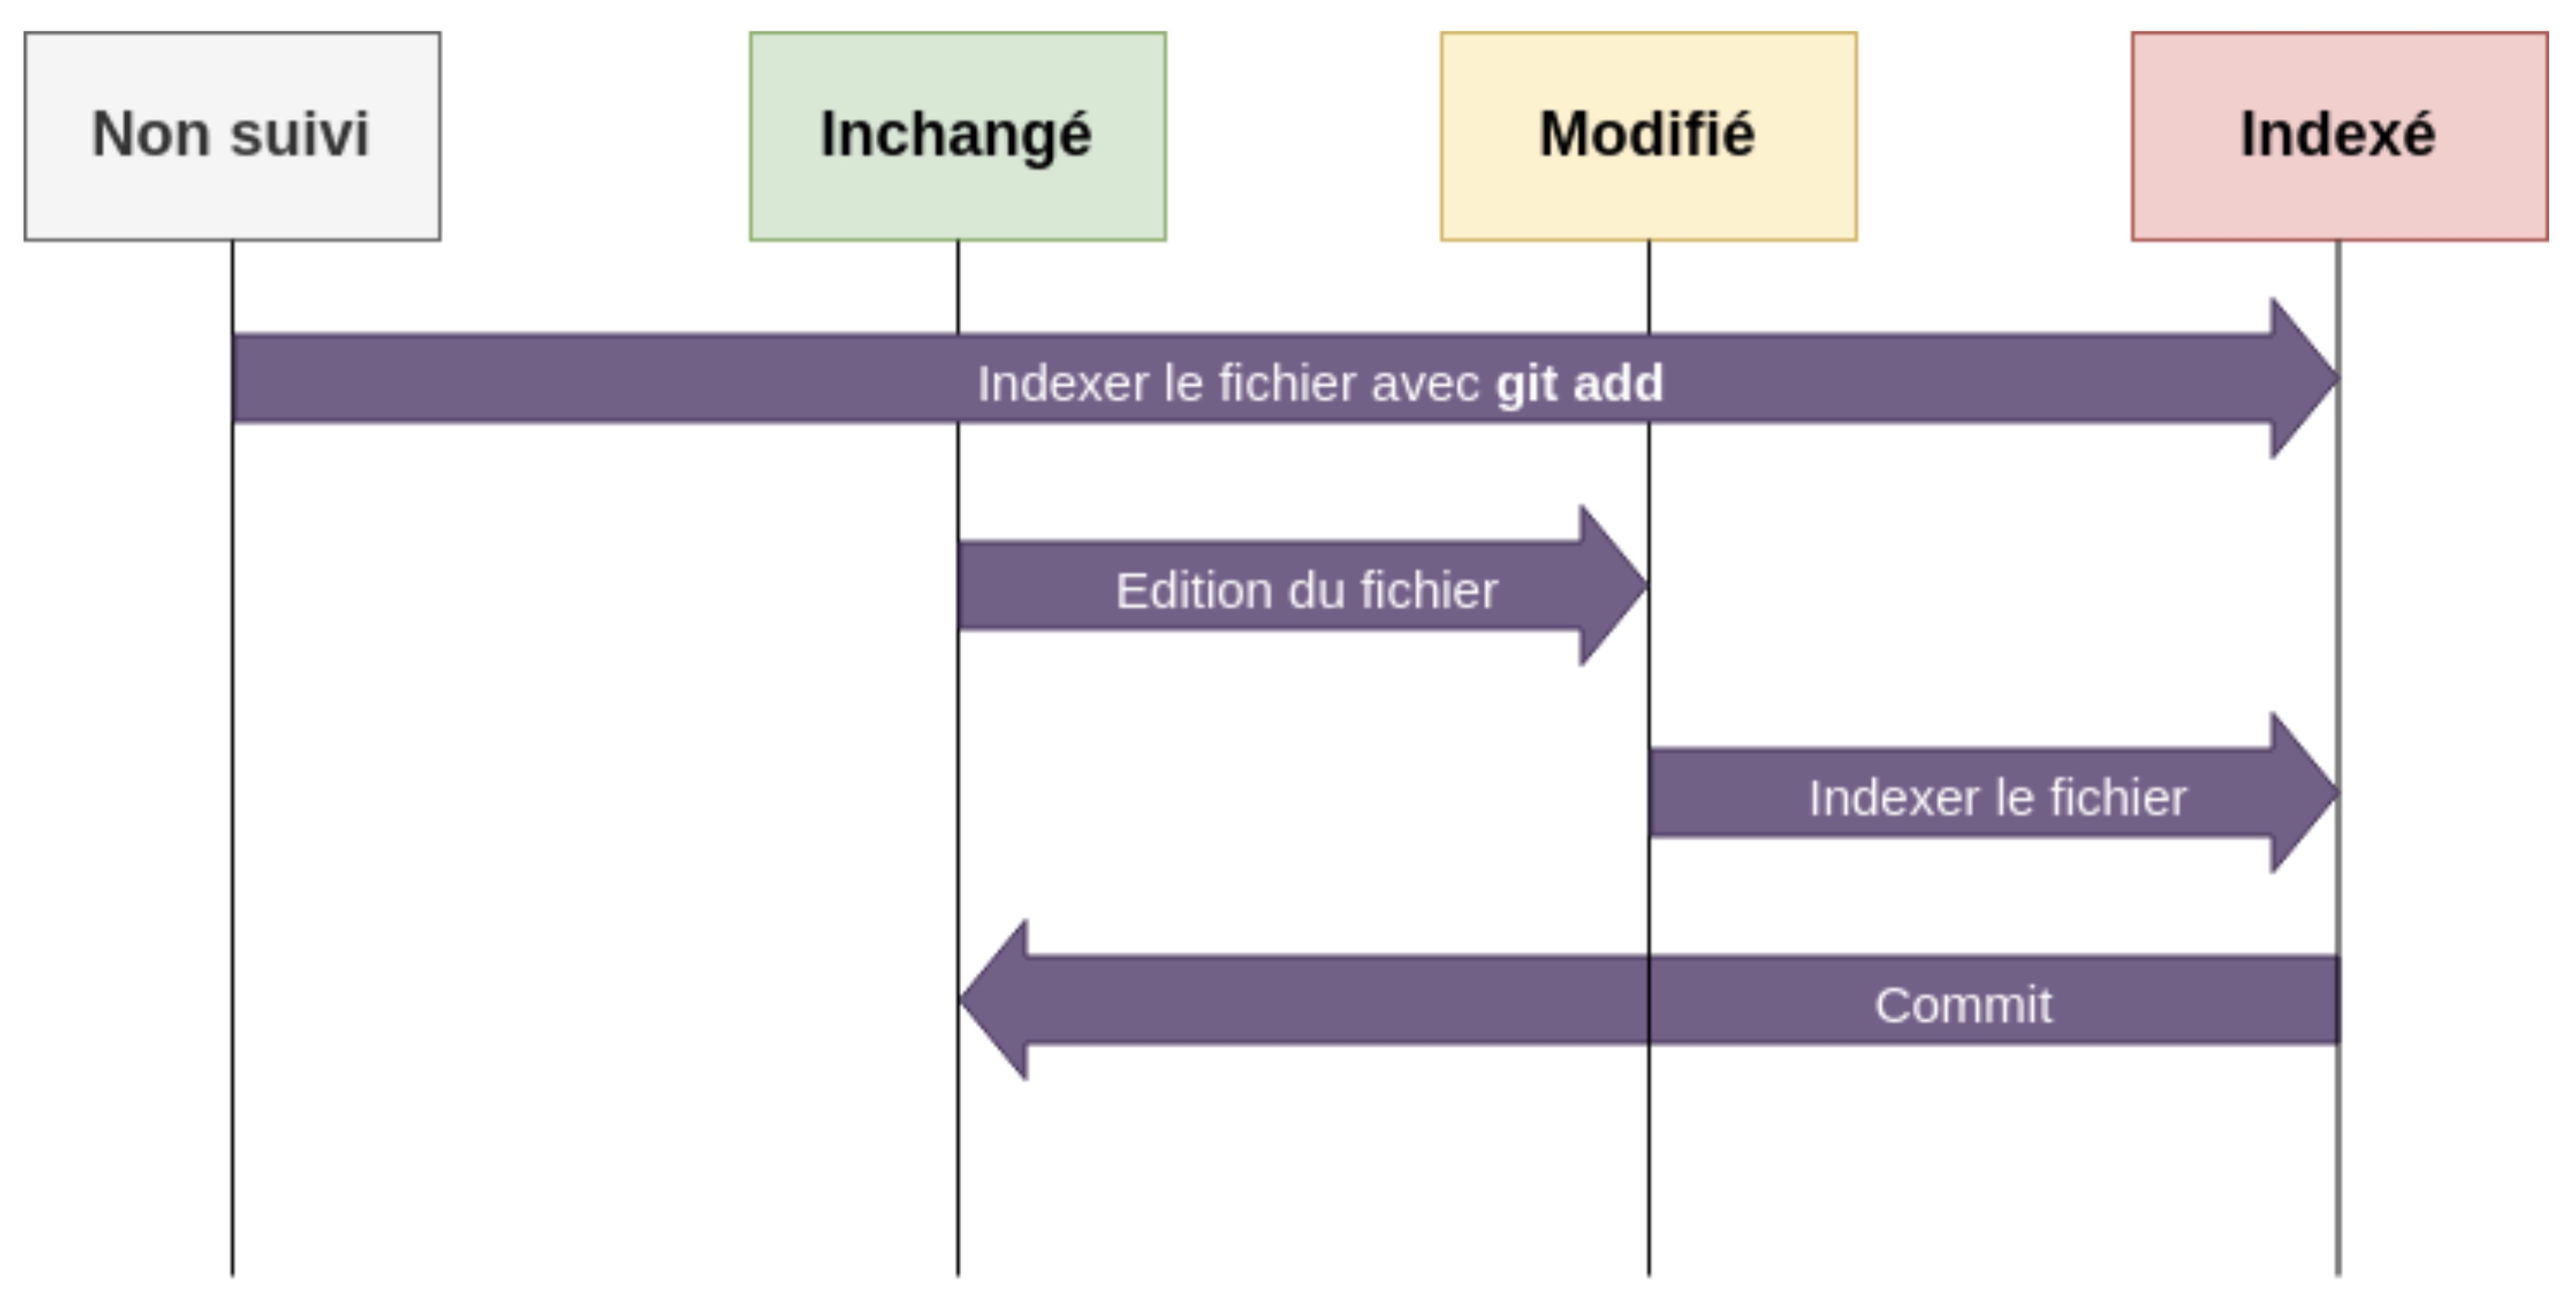
\includegraphics[scale=0.13]{image01.png} 
\end{center}


Les fichiers ne sont pas automatiquement suivis par {\color{blue} Git}, même s'il les détecte car vous pouvez vouloir ne pas suivre certains fichiers avec {\color{blue} Git} comme nous le verrons. {\color{blue} Git} vous laisse donc très libre et vous permet de choisir quels fichiers et dossiers suivre.

\section{État d'un fichier et fonctionnement de l'index}
\subsection{Les trois états possibles des fichiers}
Lorsqu'un fichier est suivi par {\color{blue} Git}, il peut être dans trois états :
\begin{enumerate}
\item  modifié : le fichier est modifié mais la version modifiée n'est pas encore indexée ou sauvegardée.

\item  indexé : le fichier est suivi par {\color{blue} Git} et ajouté en zone de transit ({\color{blue}staging area}). {\color{blue}Git} utilise, comme nous le verrons en détails, un fichier d'{\color{blue}index} pour déterminer quels fichiers feront parties de la prochaine sauvegarde.

\item  validé : le fichier est stocké dans la base de données locale {\color{blue} Git}, qui constitue avec les fichiers de configuration le dépôt local.
\end{enumerate}


Nous allons bien sûr voir ces états en détails et comment passer les fichiers d'un état à un autre.

\subsection{Le répertoire de travail ({\color{blue}working directory})}

Le répertoire de travail est la version des fichiers sur laquelle vous travaillez actuellement : autrement dit c'est l'ensemble des fichiers et des dossiers ouverts actuellement dans votre éditeur de code.

Lorsque vous changez de version en utilisant {\color{blue} Git}, vous modifiez le répertoire de travail et {\color{blue} Git} extrait la bonne version des fichiers de sa base de données.

\subsection{Indexer un fichier dans la zone de transit ({\color{blue}staging area})}
Un fichier indexé est un fichier qui est en zone de transit et qui sera ajouté à la prochaine sauvegarde effectuée avec {\color{blue} Git}. Pour indexer un fichier ou un dossier avec {\color{blue} Git}, il faut utiliser la commande :

\begin{minted}[
%frame=lines,
framesep=2mm,
baselinestretch=1.2,
bgcolor=LightGray,
fontsize=\footnotesize,
% linenos
]{shell}
git add fichier|dossier
\end{minted}

Le fichier ou le dossier (et tous les fichiers et dossiers qu'il contient éventuellement) seront alors indexés et suivis par {\color{blue} Git}. Nous allons donc indexer le fichier de test que nous avons créé pour voir ce qu'il se passe :

\begin{minted}[
%frame=lines,
framesep=2mm,
baselinestretch=1.2,
bgcolor=LightGray,
fontsize=\footnotesize,
% linenos
]{shell}
git add test.txt
\end{minted}

Ensuite nous regardons où en est {\color{blue} Git} en faisant ;

\begin{minted}[
%frame=lines,
framesep=2mm,
baselinestretch=1.2,
bgcolor=LightGray,
fontsize=\footnotesize,
% linenos
]{shell}
git status
\end{minted}

{\color{blue} Git} nous indique que nous sommes toujours sur la branche master et que nous n'avons aucun commit. Mais à la différence d'avant, nous avons :

\begin{verbatim}
Modifications qui seront validées : nouveau fichier : test.txt.
\end{verbatim}

{\color{blue} Git} nous dit ici que le fichier est bien indexé. Il apparaît d'ailleurs en vert (alors qu'avant il était en rouge). Le fichier est maintenant en zone de transit ({\color{blue} staging area}), c'est-à-dire qu'il fera partie de la prochaine sauvegarde que nous effectuerons avec {\color{blue} Git}. Approfondissons sur ce que {\color{blue} Git} a fait. Tapez la commande :

\begin{minted}[
%frame=lines,
framesep=2mm,
baselinestretch=1.2,
bgcolor=LightGray,
fontsize=\footnotesize,
% linenos
]{shell}
git ls-files --stage
\end{minted}

Cette commande permet d'obtenir des informations sur les fichiers contenu dans le répertoire local ou dépôt local suivi par {\color{blue} Git}. En passant l'option stage, nous obtenons les informations sur les fichiers qui sont dans la zone de transit (staging area). Ces informations se trouvent en fait dans le fichier .git/index, mais en binaire. La commande permet donc de les rendre lisible :

\begin{verbatim}
100644 ac28f91b8c7314ce04f3f037948520dcc7a88ff7 0	test.txt
\end{verbatim}
\begin{itemize}
\item Le premier nombre contient les bits de permissions et de type de fichier. Nous n'allons pas aller trop loin car c'est bas niveau. Sachez qu'ici {\color{blue} 100} signifie fichier standard et {\color{blue} 644} fichier que l'utilisateur propriétaire ({\color{blue} owner}) peut lire et écrire mais pas exécuter (et que le groupe et les autres ne peuvent que lire).

\item La deuxième partie est la somme de contrôle {\color{blue} SHA-1} du fichier, appelé {\color{blue} hash} comme nous l'avons vu.

\item Le troisième nombre est utilisé pour la fusion (nous la verrons plus tard dans le cours). Il est très important pour la gestion des conflits.

\item La dernière partie est le nom du fichier.
\end{itemize}


Mais que contient exactement le fichier {\color{blue} .git/index} ? Comme dit précédemment il contient du binaire. Mais nous pouvons l'afficher en hexadécimal :

\begin{minted}[
%frame=lines,
framesep=2mm,
baselinestretch=1.2,
bgcolor=LightGray,
fontsize=\footnotesize,
% linenos
]{shell}
hexdump .git/index
\end{minted}

hexdump permet d'afficher dans la sortie standard, ici le terminal, un hexadecimal dump, c'est-à-dire d'afficher les données binaires du fichier en hexadécimal.

Ce qui donne quelque chose comme ça :
\begin{center}
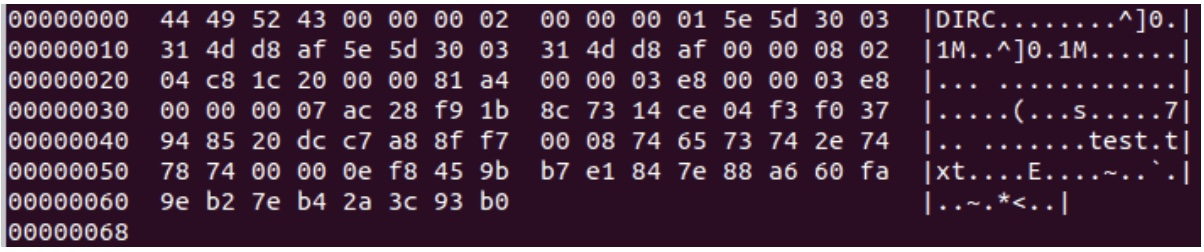
\includegraphics[scale=0.25]{image02.jpg} 
\end{center}

Dans ces informations il y a : la version de {\color{blue} Git} utilisée, la dernière fois que le fichier a été modifié ({\color{blue} timestamp}), le disque dur sur lequel se trouve le fichier (en l'occurence {\color{blue} test.txt}), l'{\color{blue} inode} du fichier (identifiant unique du fichier et informations systèmes bas niveau sur le fichier), les permissions du fichier (qui peut le lire, y écrire ou l'exécuter), le chemin vers le fichier, les identifiants de l'utilisateur et du groupe courant, la taille du fichier et bien sûr la somme de contrôle {\color{blue} SHA-1}, ou {\color{blue} hash}.

Vous n'aurez bien évidemment jamais à accéder à ce fichier, qui est uniquement un fichier d'administration utilisé par {\color{blue} Git}. Mais cela vous permet d'avoir déjà une bonne idée des informations qu'il contient.

\subsection{Modification d'un fichier suivi}
Modifions maintenant notre fichier {\color{blue} text.txt} pour observer le comportement de {\color{blue} Git} :


\begin{minted}[
%frame=lines,
framesep=2mm,
baselinestretch=1.2,
bgcolor=LightGray,
fontsize=\footnotesize,
% linenos
]{shell}
nano text.txt
\end{minted}

L'éditeur {\color{blue} nano} est un un éditeur libre du système {\color{blue} GNU}. Il suffit de l'installer si le terminal vous indique que la commande n'est pas connue :


\begin{minted}[
%frame=lines,
framesep=2mm,
baselinestretch=1.2,
bgcolor=LightGray,
fontsize=\footnotesize,
% linenos
]{shell}
apt-get install nano
\end{minted}

Mettez par exemple {\color{blue} Coucou2}, sauvegardez ({\color{blue} ctrl + o} puis entrée) et quittez ({\color{blue} ctrl + x}). Refaites un :

\begin{minted}[
%frame=lines,
framesep=2mm,
baselinestretch=1.2,
bgcolor=LightGray,
fontsize=\footnotesize,
% linenos
]{shell}
git status
\end{minted}

Qu'obtenons-nous ? Les informations sur la branche et le {\color{blue} commit} n'ont pas changé. Nous avons des modifications qui seront validées (en {\color{blue} vert}) :

\begin{verbatim}
nouveau fichier : test.txt
\end{verbatim}

Et nouveauté, des modifications qui ne seront pas validées (en rouge) :

\begin{verbatim}
modifié :         test.txt
\end{verbatim}

Intéressant ! Cela signifie qu'une fois qu'un nouveau fichier a été indexé, si nous le modifions ensuite, la nouvelle modification n'est pas ajoutée à l'{\color{blue} index} !

Il faut refaire {\color{blue} git add test.txt} pour indexer la modification pour la prochaine sauvegarde :


\begin{minted}[
%frame=lines,
framesep=2mm,
baselinestretch=1.2,
bgcolor=LightGray,
fontsize=\footnotesize,
% linenos
]{shell}
git add test.txt
\end{minted}

Et maintenant la nouvelle modification est bien indexée par {\color{blue} Git} :

\begin{verbatim}
nouveau fichier : test.txt
\end{verbatim}
\begin{itemize}
\item Il faut donc bien retenir que {\color{blue} Git} détecte les fichiers qui ne sont pas suivis dans le dépôt et les modifications effectuées sur les fichiers.

\item Cependant, par défaut, {\color{blue} Git} ne va pas indexer et mettre ces nouveaux fichiers, ou ces fichiers modifiés, en zone de transit (staging area).

\item La raison est simple : {\color{blue} Git} vous laisse totalement libre pour indiquer quels fichiers et quelles modifications des fichiers doivent être ajoutées à la prochaine sauvegarde.
\end{itemize}


Maintenant que vous savez ça, reprenez le schéma vu dans la leçon précédente et il devrait être un peu plus clair ! Il le sera encore plus une fois que nous aurons étudié les {\color{blue} commits}.

Retenez que {\color{blue} git add} permet en fait d'ajouter la version actuelle d'un fichier à la prochaine sauvegarde.

Cela signifie que si vous modifiez une nouvelle fois test.txt après l'avoir {\color{blue} git add}, la nouvelle version du fichier ne sera pas indexée et ne sera pas mise en zone de transit ({\color{blue} staging area}). Il faudra de nouveau le {\color{blue} git add} si vous voulez inclure la dernière version dans la sauvegarde.

A notez que comme nous l'avons déjà dit, si vous ajoutez un dossier, alors tous les fichiers et les dossiers contenus dans ce dossier seront indexés et mis en zone de transit.

\section{Ignorer des fichiers et des dossiers}
\subsection{Ignorer des fichiers}
Dans tous les projets que vous ferez, il y a des fichiers et des dossiers que vous ne voudrez pas du tout suivre avec Git. Vous ne voudrez pas que {\color{blue} Git}  sauvegarde différentes versions de ces fichiers et dossiers.

Pour ignorer des fichiers, il faut créer un fichier spécial à la racine de votre projet, pour nous, dans le dossier {\color{blue} test-git} :

\begin{minted}[
%frame=lines,
framesep=2mm,
baselinestretch=1.2,
bgcolor=LightGray,
fontsize=\footnotesize,
% linenos
]{shell}
nano .gitignore
\end{minted}

Ce fichier est un fichier caché, et c'est pour cette raison qu'il commence par un point. Dans ce fichier vous mettrez souvent le dossier des dépendances {\color{blue} node\_modules}, les fichiers de configuration de votre éditeur de code, des fichiers de log en local etc. Par exemple nous pouvons simplement mettre :

\begin{verbatim}
node\_modules
\end{verbatim}

Tous les dossiers (et leur contenu) et les fichiers s'appelant {\color{blue}node\_modules} seront ignorés par {\color{blue} Git} . Si vous terminez un nom avec /, seuls les dossiers (et tout leur contenu) avec le nom spécifié seront ignorés, par exemple :

\begin{verbatim}
node\_modules/
\end{verbatim}

Vous pouvez également utiliser des expressions régulières simplifiées dans ce fichier. {\color{blue} *} signifie un ou plusieurs caractères :

\begin{verbatim}
local-doc/*.txt
\end{verbatim}

Ici, tous les fichiers qui sont dans un dossier {\color{blue}local-doc} et qui finissent par {\color{blue}.txt} seront ignorés. Ainsi par exemple le fichier {\color{blue}/projet/local/local-doc/test.txt} serait ignoré. En revanche, {\color{blue}/projet/local/local-doc/commands/test.txt} ne sera pas ignoré car il est dans un sous-dossier. {\color{blue}**} signifie une série d'un ou plusieurs dossiers : Ainsi, pour ignorer tous les fichiers dans le dossier et les sous-dossiers qui finissent par {\color{blue}.txt}, il faut faire :

\begin{verbatim}
local-doc/**/*.txt
\end{verbatim}

Ici tous les fichiers finissant par {\color{blue}.txt} et qui sont dans le dossier {\color{blue}local-doc} ou dans un dossier situé dans {\color{blue}local-doc} (même sur plusieurs niveaux de dossiers) seront ignorés.

\section{Afficher les différences entre répertoire, index et sauvegarde avec git diff}
\subsection{Vérifier les fichiers indexés, modifiés et non indexés}
Nous avons vu que la commande {\color{blue}git status} nous donnait certaines informations sur les fichiers indexés.

Nous allons voir qu'il existe une autre commande permettant d'obtenir plus d'informations sur les fichiers indexés en zone de transit ({\color{blue}staging area}) : {\color{blue}git diff}.

\subsection{Afficher les modifications des fichiers non indexés}
La commande {\color{blue}git diff} sans aucune option permet d'afficher les modifications des fichiers dans le répertoire de travail qui ont été modifiés mais non indexés. En fait, elle permet de comparer les fichiers du répertoire de travail avec la zone de transit, c'est-à-dire avec les fichiers indexés, et de n'afficher que les fichiers qui ont donc des modifications non indexées.

Si vous tapez {\color{blue}git diff} maintenant, vous n'aurez rien car nous n'avons avons indexé le fichier {\color{blue}test.txt} que nous avons modifié. Modifions de nouveau le fichier :

\begin{minted}[
%frame=lines,
framesep=2mm,
baselinestretch=1.2,
bgcolor=LightGray,
fontsize=\footnotesize,
% linenos
]{shell}
nano text.txt
\end{minted}

Mettez par exemple {\color{blue}Coucou3}, sauvegardez ({\color{blue}ctrl + o} puis entrée) et quittez ({\color{blue}ctrl + x}). Refaites un :

\begin{minted}[
%frame=lines,
framesep=2mm,
baselinestretch=1.2,
bgcolor=LightGray,
fontsize=\footnotesize,
% linenos
]{shell}
git diff
\end{minted}

Vous aurez le résultat suivant, que nous allons voir ensemble :
\begin{verbatim}
diff --git a/test.txt b/test.txt
index ae362e4..1344bd0 100644
--- a/test.txt
+++ b/test.txt
@@ -1 +1 @@
-Coucou2
+Coucou3
\end{verbatim}

La première ligne {\color{blue}diff --git} permet de spécifier que nous sommes au format {\color{blue}git diff} et {\color{blue}a/test.txt} {\color{blue}b/test.txt} permet de spécifier qu'il y a des différences entre le fichier indexé et le fichier dans le répertoire de travail.

La seconde ligne nous donnes le début du {\color{blue}hash} de la version du fichier indexée, puis {\color{blue}…} et le début du {\color{blue}hash} de la version du fichier dans le répertoire de travail. Nous avons ensuite {\color{blue}100644} qui comme nous l'avions vu donne le type de fichier et les permissions ({\color{blue}644}).

Ensuite nous avons deux lignes qui nous donne quels fichiers ont été modifiés, il y a toujours {\color{blue}---} et {\color{blue}+++} quel que soit le nombre de modifications entre les deux versions du fichier.

Ensuite nous avons {\color{blue}@@ -1 +1 @@}. Il permet de spécifier les intervalles de lignes dans le fichier où il y a des différences entre les deux versions.
\begin{enumerate}
\item Le premier nombre précédé par un {\color{blue}-} permet de spécifier la ligne de départ des différences (ici la ligne 1) dans la version de départ, puis il est éventuellement suivi d'une virgule et d'un autre nombre qui signifie jusqu'à la ligne n.

\item Le second nombre, précédé par un {\color{blue}+} est le même intervalle de lignes dans le fichiers pour les différences mais pour la version d'arrivée.
\end{enumerate}

Ici, cela signifie que nous avons des différences uniquement sur la première ligne dans le fichier de départ et dans le fichier d'arrivée. Remodifions le fichier test.txt pour avoir un exemple plus complet :


\begin{minted}[
%frame=lines,
framesep=2mm,
baselinestretch=1.2,
bgcolor=LightGray,
fontsize=\footnotesize,
% linenos
]{shell}
nano text.txt
\end{minted}

Mettez par exemple {\color{blue}Test} à la seconde ligne et {\color{blue}Test2} à la troisième ligne, sauvegardez ({\color{blue}ctrl + o} puis entrée) et quittez ({\color{blue}ctrl + x}). Refaites un :

\begin{minted}[
%frame=lines,
framesep=2mm,
baselinestretch=1.2,
bgcolor=LightGray,
fontsize=\footnotesize,
% linenos
]{shell}
git diff
\end{minted}

Nous avons maintenant :

\begin{verbatim}
diff --git a/test.txt b/test.txt
index ae362e4..01e8afb 100644
--- a/test.txt
+++ b/test.txt
@@ -1 +1,3 @@
-Coucou2
+Coucou3
+Test
+Test2
\end{verbatim}

Nous voyons que l'intervalle de départ est toujours de la première ligne à la première ligne ({\color{blue}1,1} est abrégé en {\color{blue}1}) ce qui signifie que dans la version de départ la première ligne diffère par rapport à la version d'arrivée.

En revanche, pour l'intervalle d'arrivée, nous avons {\color{blue}1,3} ce qui signifie que nous avons des différences de la première à la troisième ligne dans le fichier d'arrivée.

Enfin, nous avons la liste des différences entre les deux fichiers précédés par des {\color{blue}-} pour les suppressions et par des {\color{blue}+} pour les ajouts.

\subsection{Afficher les modifications des fichiers indexés}
La commande {\color{blue}git diff --staged} permet d'afficher les modifications des fichiers indexés par rapport à la dernière sauvegarde. Cette commande compare les différences entre la dernière sauvegarde (ou l'origine si il n'y a eu aucune sauvegarde) et l'index. Elle permet de visualiser les différences qui seront donc sauvegardées par {\color{blue}Git} :

\begin{minted}[
%frame=lines,
framesep=2mm,
baselinestretch=1.2,
bgcolor=LightGray,
fontsize=\footnotesize,
% linenos
]{shell}
git diff --staged
\end{minted}

Ici, dans notre exemple, nous avons :

\begin{verbatim}
diff --git a/test.txt b/test.txt
new file mode 100644
index 0000000..ae362e4
--- /dev/null
+++ b/test.txt
@@ -0,0 +1 @@
+Coucou2
\end{verbatim}

En effet, nous avons les différences entre l'origine et la version du fichier que nous avions indexée. 
\begin{itemize}
\item Nous avons la même chose pour la première ligne.

\item La seconde ligne indique que nous avons créé un fichier standard avec les permissions {\color{blue}644}.

\item La troisième ligne indique {\color{blue}0000000} car il n'y a pas de version précédente du fichier vu que nous l'avons créé et il n'y a donc pas de {\color{blue}hash} de départ. {\color{blue}ae362e4} est le début du {\color{blue}hash} de la version du fichier indexée.

\item Ensuite, nous avons {\color{blue}$-$$-$$-$ /dev/null} qui signifie que la source du fichier est {\color{blue}null} car nous le créons. (Si nous supprimions un fichier nous aurions {\color{blue}+++ /dev/null} car c'est la cible qui deviendrait {\color{blue}null}).

\item {\color{blue}@@ $-0$,0 +1 @@} signifie que nous n'avions pas de fichier donc l'intervalle de départ est de la ligne 0 à 0 et l'intervalle d'arrivée est {\color{blue}1} qui signifie que nous avons une différence à la ligne {\color{blue}1} avec le fichier d'origine (qui est inexistant ici).

\item Enfin, nous avons la différence qui est affichée : {\color{blue}+Coucou2}. Nous avons ajouté {\color{blue}Coucou2}.

\end{itemize}
Rappelez-vous bien que la comparaison des différences est ici entre la dernière sauvegarde ou l'origine et les fichiers dans la zone de transit, c'est-à-dire indexé.

C'est pour cette raison que nous n'avons pas {\color{blue}Coucou1} ou autre chose, car nous n'avons pas de sauvegarde donc l'origine est {\color{blue}null}.

\section{Créer des sauvegardes avec git commit}
\subsection{Créer une sauvegarde}
En {\color{blue}Git}, nous parlons de validation des modifications pour une sauvegarde. Une sauvegarde s'appelle un commit, cela signifie littéralement que nous engageons les modifications indexées.

Un commit n'est donc pas à prendre à la légère ! C'est une sauvegarde qui sera à tout jamais dans le dépôt {\color{blue}Git}.

\subsubsection*{La commande git commit}
Pour faire un commit, il suffit de taper :

\begin{minted}[
%frame=lines,
framesep=2mm,
baselinestretch=1.2,
bgcolor=LightGray,
fontsize=\footnotesize,
% linenos
]{shell}
git commit
\end{minted}

{\color{blue}Git} va alors ouvrir l'éditeur par défaut, si vous rencontrez cette erreur :

\begin{verbatim}
hint: Waiting for your editor to close the file... error: unable to start editor 'editor'
\end{verbatim}

Cela veut dire que {\color{blue}Git} ne sait pas quel éditeur utiliser. Dans ce cas, nous allons le configurer :

\begin{minted}[
%frame=lines,
framesep=2mm,
baselinestretch=1.2,
bgcolor=LightGray,
fontsize=\footnotesize,
% linenos
]{shell}
git config --system core.editor nano
\end{minted}

Ici nous mettons en configuration système, la plus haut niveau, que nous utiliserons l'éditeur {\color{blue}nano}. Refaites la commande : {\color{blue}git commit} ensuite. Vous aurez alors :

\begin{verbatim}
# Veuillez saisir le message de validation pour vos modifications. Les lignes
# commençant par '#' seront ignorées, et un message vide abandonne la validation.
#
# Sur la branche master
#
# Validation initiale
#
# Modifications qui seront validées :
#       nouveau fichier : test.txt
#
# Modifications qui ne seront pas validées :
#       modifié :         test.txt
#
\end{verbatim}
Nous avons un résumé de ce qui va être sauvegardé. Comme prévu, la version indexée du fichier {\color{blue}test.txt} va être sauvegardée, mais pas la version modifiée de ce fichier que nous n'avons pas indexé. Fermez l'éditeur en faisant {\color{blue}ctrl + x}. Vous aurez le message suivant :
\begin{verbatim}
Abandon de la validation dû à un message de validation vide.
\end{verbatim}
C'était pour vous montrer que les sauvegardes sur {\color{blue}Git} doivent obligatoirement avoir un message de validation, c'est-à-dire un court texte décrivant les changements apportés dans cette version.

Nous allons ajouter une option afin de vérifier exactement ce que nous avons modifié :

\begin{minted}[
%frame=lines,
framesep=2mm,
baselinestretch=1.2,
bgcolor=LightGray,
fontsize=\footnotesize,
% linenos
]{shell}
git commit -v
\end{minted}

Cela permet en fait de mettre le résultat de {\color{blue}git diff --staged} après le commentaire dans l'éditeur :
\begin{verbatim}
# Veuillez saisir le message de validation pour vos modifications. Les lignes
# commençant par '#' seront ignorées, et un message vide abandonne la validation.
#
# Sur la branche master
#
# Validation initiale
#
# Modifications qui seront validées :
#       nouveau fichier : test.txt
#
# Modifications qui ne seront pas validées :
#       modifié :         test.txt
#
# ------------------------ >8 ------------------------
# Ne touchez pas à la ligne ci-dessus.
# Tout ce qui suit sera éliminé.
diff --git a/test.txt b/test.txt
new file mode 100644
index 0000000..ae362e4
--- /dev/null
+++ b/test.txt
@@ -0,0 +1 @@
+Coucou2

\end{verbatim}
Nous vous encourageons à le faire au début pour bien vérifier ce que vous allez sauvegarder. Quittez l'éditeur avec {\color{blue}ctrl + x}.

\subsubsection*{Le message de commit}
Pour l'instant nous n'avons rien sauvegardé, car nous avons à chaque fois abandonné le {\color{blue}commit} en ne précisant pas de message de validation. Nous allons le refaire une fois, mais en ajoutant à la première ligne le message suivant : {\color{blue}Premier commit}. Puis nous allons sauvegarder {\color{blue}ctrl + o} et quittez {\color{blue}ctrl + x}. Nous avons alors le message suivant :
\begin{verbatim}
[master (commit racine) bfc88f2] Premier commit
1 file changed, 1 insertion(+)
create mode 100644 test.txt
\end{verbatim}

Nous avons effectué notre première sauvegarde dans {\color{blue}Git} ! Notez que seul le message spécifié est enregistré dans le commit, si les commentaires, ni le résultat de {\color{blue}git diff --staged} en utilisant {\color{blue}git commit -v} n'ont été sauvegardés.

La première ligne nous indique d'abord la branche sur laquelle nous avons effectué le {\color{blue}commit}, ici {\color{blue}master} (nous reviendrons très en détails sur les branches plus tard). Ensuite un message indique qu'il s'agit du premier commit, appelé {\color{blue}root commit} ou {\color{blue}commit} racine. Nous retrouvons le début du {\color{blue}hash} du {\color{blue}commit}, ainsi que le début du message de validation, appelé également message de {\color{blue}commit}.

Enfin, nous retrouvons un résumé de ce que nous avons fait : nous avons modifié un seul fichier, que nous avons créé avec les permissions par défaut ({\color{blue}create mode 100644 test.txt}) et effectué une insertion d'une ligne

\subsubsection*{Recommandations sur les messages de commit}
Il est recommandé par {\color{blue}Git} d'effectuer des messages de validation décomposé de la manière suivante :
\begin{itemize}
\item 1ère ligne : titre du commit de moins de 50 caractères qui résume la modification.
\item Puis une seconde ligne vide (saut de ligne).
\item Puis un paragraphe décrivant de façon plus précise les modifications apportées.
\end{itemize}
Voici par exemple un message de commit du répertoire de {\color{blue}Git} sur Github (oui {\color{blue}Git} est développé en utilisant comme système de version… lui-même, c'est une belle mise en abîme).

\begin{verbatim}
Azure Pipeline: switch to the latest agent pools

It would seem that at least the `vs2015-win2012r2` pool (which we use
via its old name, `Hosted`) is about to be phased out. Let's switch
before that.
\end{verbatim}

\subsubsection*{Le raccourci {\color{blue}git commit -m}}
Lorsque vous serez un peu plus familier de {\color{blue}git}, nous allons utiliser {\color{blue}git commit -m} qui permet de ne pas ouvrir l'éditeur et directement de passer le message de validation.

Afin de respecter la recommandation il faut utiliser un premier -m pour le titre et un second pour le corps. Ajoutons les modifications que nous n'avions pas indexé :

\begin{minted}[
%frame=lines,
framesep=2mm,
baselinestretch=1.2,
bgcolor=LightGray,
fontsize=\footnotesize,
% linenos
]{shell}
git add test.txt
\end{minted}

Puis vérifions ce qui va être sauvegardé :

\begin{minted}[
%frame=lines,
framesep=2mm,
baselinestretch=1.2,
bgcolor=LightGray,
fontsize=\footnotesize,
% linenos
]{shell}
git diff --staged
\end{minted}

Et nous obtenons :
\begin{verbatim}
diff --git a/test.txt b/test.txt
index ae362e4..de0e405 100644
--- a/test.txt
+++ b/test.txt
@@ -1 +1,3 @@
  Coucou2
+Test
+Test2
\end{verbatim}

Nous effectuons maintenant le {\color{blue}commit} en suivant les recommandations sur les messages de validation :


\begin{minted}[
%frame=lines,
framesep=2mm,
baselinestretch=1.2,
bgcolor=LightGray,
fontsize=\footnotesize,
% linenos
]{shell}
git commit -m "Second commit de test" 
  -m "Nous avons ajouté deux lignes dans notre fichier test.txt afin de tester le comportement 
  de Git lorsque nous modifions plusieurs lignes"
\end{minted}

Nous avons notre titre en premier, puis le descriptif avancé en second.

\subsection{Sauter l'étape de la zone transitoire (ou indexation)}
Parfois vous souhaiterez faire une petite modification et vous n'aurez pas besoin de contrôler ce que vous allez sauvegarder, et vous ne voudrez pas non plus indexer manuellement ces modifications avec {\color{blue}git add}. Dans ce cas vous pouvez utiliser l'option {\color{blue}git commit -a}.

Reprenons notre exemple en modifiant le fichier test.txt une nouvelle fois :


\begin{minted}[
%frame=lines,
framesep=2mm,
baselinestretch=1.2,
bgcolor=LightGray,
fontsize=\footnotesize,
% linenos
]{shell}
nano test.txt
\end{minted}

Supprimez par exemple une ligne, sauvegardez ({\color{blue}ctrl + o}) et quittez ({\color{blue}ctrl + x}). Nous utilisons maintenant le raccourci :

\begin{minted}[
%frame=lines,
framesep=2mm,
baselinestretch=1.2,
bgcolor=LightGray,
fontsize=\footnotesize,
% linenos
]{shell}
git commit -am "Suppression de la dernière ligne" 
-m "Nous supprimons la dernières ligne pour tester l'indexation automatique des fichiers suivis."
\end{minted}

Nous n'avons pas eu à indexer le fichier avec {\color{blue}git add} après la modification. {\color{blue}Git} l'a fait automatiquement pour nous.

A noter que {\color{blue}Git} n'indexera automatiquement que les fichiers qui sont suivis.

Si vous avez des fichiers créés mais non encore suivi, ils ne seront donc pas sauvegardés dans le commit !

\subsection{Les informations contenues dans un {\color{blue}commit}}
Les informations suivantes, appelées métadonnées (c'est-à-dire des données informatives sur d'autres données), sont enregistrées dans un objet {\color{blue}commit }:
\begin{itemize}
\item Nom et email l'auteur du code : c'est l'auteur des modifications (celui qui a écrit le code).

\item Nom et email du {\color{blue}committer} : le {\color{blue}committer} est celui qui effectue le commit de fusion (nous verrons la fusion plus tard). La plupart du temps l'{\color{blue}author} et le {\color{blue}committer} sont les mêmes personnes.

Mais sur certains projets importants, il y a une étape de validation pour chaque {\color{blue}commit}, les auteurs du code envoient souvent leurs {\color{blue}patch} (leurs {\color{blue}commits} de modifications) par email (pour {\color{blue}Linux} ou {\color{blue}Git} par exemple, ou comme nous le verrons sur {\color{blue}Github/Gitlab}), aux {\color{blue}reviewers} (qui relisent le code) et ce sont ces contributeurs de l'équipe {\color{blue}core} qui vont effectuer le {\color{blue}commit}, c'est-à-dire valider les modifications à sauvegarder. Dans ce cas, il y aura un commit de fusion et ce cera le {\color{blue}reviewer} qui sera le {\color{blue}committer}.

\item Il y a ensuite la date des modifications ({\color{blue}GIT\_AUTHOR\_DATE}) et la date du commit ({\color{blue}GIT\_COMMITTER\_DATE}).

\item Il y a également le {\color{blue}hash} du tree racine de l'instantané, nous allons détailler juste après.

\item Et enfin, le {\color{blue}hash} du commit parent, nous détaillerons également.

\item Ensuite, {\color{blue}Git} génère le {\color{blue}hash} de toutes ces informations avec l'algorithme {\color{blue}SHA-1} ce qui nous donne le {\color{blue}hash} du commit.

Le {\color{blue}hash} permet de s'assurer de l'intégrité de toutes ces métadonnées. Aucune donnée ne pourra être modifiée sans que {\color{blue}Git} ne le sache car le {\color{blue}hash} serait modifié.

\end{itemize}
\subsection{Les objets {\color{blue}Git}}
Il existe trois types d'objet {\color{blue}Git} : les blob, les commits et les trees (ou arbres). Vous pouvez afficher tous les objets de votre répertoire {\color{blue}Git} avec cette commande :

\begin{minted}[
%frame=lines,
framesep=2mm,
baselinestretch=1.2,
bgcolor=LightGray,
fontsize=\footnotesize,
% linenos
]{shell}
find .git/objects -type f
\end{minted}
\begin{itemize}
\item {\color{blue}find} est une commande permettant de rechercher des fichiers et des dossiers. Nous lui passons l'option {\color{blue}-type f} qui permet de préciser que nous recherchons que des fichiers réguliers ({\color{blue}f}).

\item {\color{blue}.git/objects} permet de préciser que nous recherchons uniquement les fichiers dans ce dossier. Nous obtenons ainsi tous les fichiers de ce dossier, ce qui donne quelque chose comme ça :
\begin{verbatim}
.git/objects/35/f8bc3582cb5f2897ccbc51d19f3bf41e748ccb
.git/objects/ac/28f91b8c7314ce04f3f037948520dcc7a88ff7
.git/objects/a5/6ccd8f89364bf9176fea2ab599b81a208ca857
.git/objects/c7/737ce0b53ff193d25019f011d265ae8201ceb3
.git/objects/1a/062bd8f48541dbfb8b3c7f5147b16fba3883e3
.git/objects/7e/8fa1f55e55b84e1339e40cdd8df8060117e6de
.git/objects/10/864573c8ec172a6377f04f4228022ecb7a1a92
.git/objects/ff/8e9239574e9bed3fd1fa4d3bcca1314f7e7107
.git/objects/f8/2c7c8e522e4a2ea086b72b5ffdfc6dd3373ae2
\end{verbatim}
\end{itemize}

\subsubsection*{Le stockage des objets}
Tous ces objets sont stockés dans le dossier {\color{blue}.git/objects} de la même manière. Chaque objet a un {\color{blue}hash} {\color{blue}SHA-1} qui sera la clé si on considère {\color{blue}Git} comme une base de données clés / valeurs.

Dans le dossier {\color{blue}.git/objects}, chaque objet est inclus dans un dossier qui a pour nom les deux premières lettres de son {\color{blue}hash} (par exemple ici {\color{blue}35}) et le nom du fichier contient les 38 caractères restants de son {\color{blue}hash} (par exemple ici {\color{blue}f8bc3582cb5f2897ccbc51d19f3bf41e748ccb)}.

La valeur de ces objets sont compressés avec la librairie {\color{blue}zlib} qui utilise l'algorithme de compression {\color{blue}defalte}. Il est possible de voir ce que contient n'importe quel objet {\color{blue}Git} avec la commande suivante :

\begin{minted}[
%frame=lines,
framesep=2mm,
baselinestretch=1.2,
bgcolor=LightGray,
fontsize=\footnotesize,
% linenos
]{shell}
git cat-file -p hash
\end{minted}

Il faut préciser les 40 caractères hexadécimaux du hash, par exemple ici :


\begin{minted}[
%frame=lines,
framesep=2mm,
baselinestretch=1.2,
bgcolor=LightGray,
fontsize=\footnotesize,
% linenos
]{shell}
git cat-file -p 35f8bc3582cb5f2897ccbc51d19f3bf41e748ccb
\end{minted}

Ce qui donne par exemple :
\begin{verbatim}
Coucou
Test
Test2
\end{verbatim}

\subsubsection*{Détails sur les types d'objets}
Nous avons vu qu'il existe trois types d'objets principaux avec {\color{blue}Git}. Pour déterminer le type d'un objet il faut faire :

\begin{minted}[
%frame=lines,
framesep=2mm,
baselinestretch=1.2,
bgcolor=LightGray,
fontsize=\footnotesize,
% linenos
]{shell}
git cat-file -t hash
\end{minted}

Avec {\color{blue}t} pour type, qui donne par exemple :

\begin{minted}[
%frame=lines,
framesep=2mm,
baselinestretch=1.2,
bgcolor=LightGray,
fontsize=\footnotesize,
% linenos
]{shell}
git cat-file -t 35f8bc3582cb5f2897ccbc51d19f3bf41e748ccb
blob
\end{minted}


Tout contenu en {\color{blue}Git} est soit un arbre soit un {\color{blue}blob}. Les {\color{blue}blobs} ({\color{blue}Binary Large Objects}) sont des objets binaires qui peuvent être n'importe quoi : des fichiers de code, des images, des vidéos etc.

Les arbres (ou {\color{blue}trees}) correspondent à un répertoire et permettent à {\color{blue}Git} de stocker plusieurs fichiers ensemble. Un arbre contient une ou plusieurs entrées, chacune étant le {\color{blue}hash} d'un {\color{blue}blob} ou d'un autre arbre avec ses droits d'accès, son type et son nom de fichier associé.

Nous allons prendre un exemple complet pour bien comprendre. Nous allons repartir d'un répertoire vide et créer un dossier et trois fichiers :
\begin{verbatim}
echo 1 > fichier1.txt
echo 2 > fichier2.txt
mkdir dossier
echo 3 > dossier/fichier3.txt
\end{verbatim}

Nous avons donc deux fichiers au premier niveau et un dossier dans lequel nous avons un fichier. Nous indexons tous ces éléments puis affichons les objets créés :


\begin{minted}[
%frame=lines,
framesep=2mm,
baselinestretch=1.2,
bgcolor=LightGray,
fontsize=\footnotesize,
% linenos
]{shell}
git add .
find .git/objects -type f
\end{minted}

Nous obtenons :
\begin{verbatim}
.git/objects/0c/fbf08886fca9a91cb753ec8734c84fcbe52c9f
.git/objects/d0/0491fd7e5bb6fa28c517a0bb32b8b506539d4d
.git/objects/00/750edc07d6415dcc07ae0351e9397b0222b7ba
\end{verbatim}
Avec la commande {\color{blue}git cat-file -t hash} pour chaque objets, nous déterminons que nous avons trois {\color{blue}blobs}. En fait, lorsque nous indexons des fichiers et des dossiers, seuls les objets pour les contenus sont créés. Nous avons ici trois objets pour les trois fichiers, avec leur {\color{blue}hash} en clé et le {\color{blue}blob} en valeur (c'est-à-dire le contenu du fichier en binaire).

Que se passe t-il si nous créons notre premier {\color{blue}commit} ?

\begin{minted}[
%frame=lines,
framesep=2mm,
baselinestretch=1.2,
bgcolor=LightGray,
fontsize=\footnotesize,
% linenos
]{shell}
git commit -m "Premier commit"
find .git/objects -type f
\end{minted}
Nous avons maintenant :
\begin{verbatim}
.git/objects/0c/fbf08886fca9a91cb753ec8734c84fcbe52c9f
.git/objects/9e/633d56381d9f0335320f22ccf3f1562d1f80d8
.git/objects/3c/dcfedb18b063a6bb4f1b43ddd73e2f88d5738a
.git/objects/d0/0491fd7e5bb6fa28c517a0bb32b8b506539d4d
.git/objects/00/750edc07d6415dcc07ae0351e9397b0222b7ba
.git/objects/1e/784b993a4dc7956c84dda1d7060c56fde32ec8
\end{verbatim}

En utilisant {\color{blue}git cat-file -t hash} pour chaque, nous déterminons que nous avons toujours trois {\color{blue}blobs} (pour les contenus des trois fichiers), mais également deux arbres (ou {\color{blue}trees}) et un {\color{blue}commit}. Mais que contient un objet arbre ? Nous allons faire la commande pour obtenir ce que contient l'objet arbre racine (pour ne pas avoir à le chercher) :


\begin{minted}[
%frame=lines,
framesep=2mm,
baselinestretch=1.2,
bgcolor=LightGray,
fontsize=\footnotesize,
% linenos
]{shell}
git cat-file -p master\^{tree}
\end{minted}
{\it 
Ne retenez pas cette commande, nous avons besoin de voir de nombreuses choses avant pour l'expliquer.} Nous obtenons :
\begin{verbatim}
040000 tree 3cdcfedb18b063a6bb4f1b43ddd73e2f88d5738a	dossier
100644 blob d00491fd7e5bb6fa28c517a0bb32b8b506539d4d	fichier1.txt
100644 blob 0cfbf08886fca9a91cb753ec8734c84fcbe52c9f	fichier2.txt
\end{verbatim}
Comme nous l'avions vu l'arbre racine contient bien le {\color{blue}hash} vers les {\color{blue}blobs} qui sont contenus dans le dossier correspondant à l'arbre (ici le dossier racine) et le {\color{blue}hash} de l'arbre correspondant au dossier.

Nous retrouvons également le type ({\color{blue}blob} ou {\color{blue}tree}), les permissions et le nom du dossier ou des fichiers. Regardons ce que nous avons dans l'arbre inclus dans l'arbre racine :


\begin{minted}[
%frame=lines,
framesep=2mm,
baselinestretch=1.2,
bgcolor=LightGray,
fontsize=\footnotesize,
% linenos
]{shell}
git cat-file -p 3cdcfedb18b063a6bb4f1b43ddd73e2f88d5738a
\end{minted}

Sans surprise nous retrouvons :
\begin{verbatim}
100644 blob 00750edc07d6415dcc07ae0351e9397b0222b7ba	fichier3.txt
\end{verbatim}
Nous avons donc :
\begin{center}
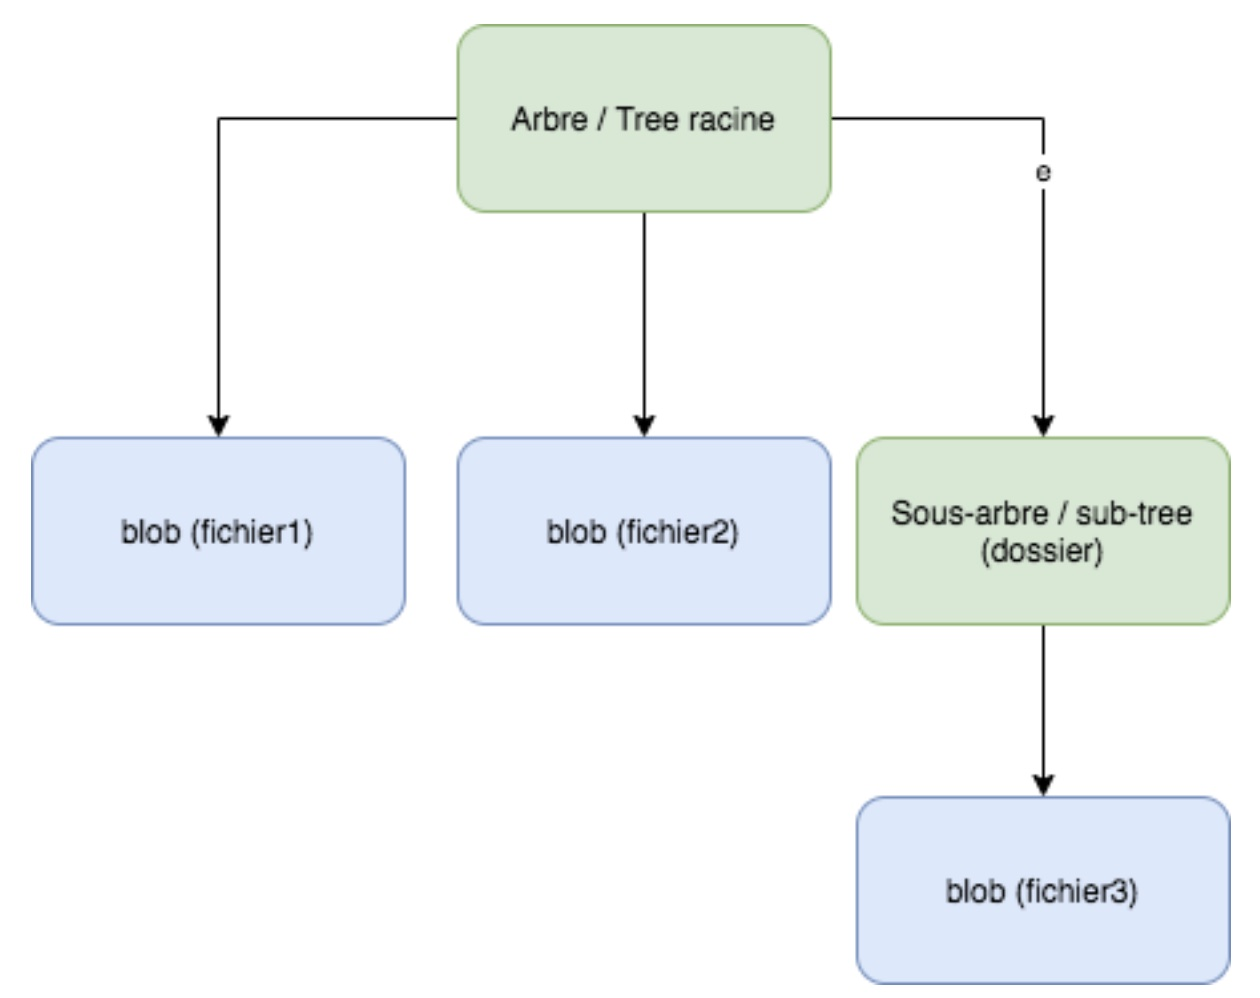
\includegraphics[scale=0.25]{image03.jpg} 
\end{center}

Nous avons vu qu'un commit créait des objets arbres pour sauvegarder un instantané d'un projet : {\color{blue}Git} enregistre toute la structure du projet grâce à ces arbres. Mais que contient l'objet commit ? C'est ce que nous allons revoir maintenant. Nous faisons la commande suivante pour ne pas avoir à rechercher le {\color{blue}hash} de l'objet commit :


\begin{minted}[
%frame=lines,
framesep=2mm,
baselinestretch=1.2,
bgcolor=LightGray,
fontsize=\footnotesize,
% linenos
]{shell}
git cat-file -p master
\end{minted}

Nous obtenons :
\begin{verbatim}
tree 1e784b993a4dc7956c84dda1d7060c56fde32ec8
author dymafr <erwanp.vallee@gmail.com> 1583754643 +0100
committer dymafr <erwanp.vallee@gmail.com> 1583754643 +0100
\end{verbatim}
Premier commit

Nous voyons que le {\color{blue}commit} contient le {\color{blue}hash} de l'arbre racine et les métadonnées que nous avions déjà vus (auteur, {\color{blue}committer}, horodatage et message de validation). Nous comprenons maintenant que grâce au {\color{blue}commit} nous avons toutes les informations d'une sauvegarde et pouvons retrouver les bonnes versions des fichiers et la bonne structure grâce à l'arbre racine inclus dans le {\color{blue}commit}.


\section{Supprimer un fichier ou un dossier}
\subsection{Effacer des fichiers avec {\color{blue}Git}}
Effaçons notre fichier de test en utilisant la commande {\color{blue}rm} (pour {\color{blue}remove}) :

\begin{minted}[
%frame=lines,
framesep=2mm,
baselinestretch=1.2,
bgcolor=LightGray,
fontsize=\footnotesize,
% linenos
]{shell}
rm test.txt
\end{minted}
Vérifions le statut de {\color{blue}Git} :

\begin{minted}[
%frame=lines,
framesep=2mm,
baselinestretch=1.2,
bgcolor=LightGray,
fontsize=\footnotesize,
% linenos
]{shell}
git status
\end{minted}
\begin{verbatim}
Nous obtenons Modifications qui ne seront pas validées : supprimé : test.txt.
\end{verbatim}
Essayons de faire un {\color{blue}commit} :

\begin{minted}[
%frame=lines,
framesep=2mm,
baselinestretch=1.2,
bgcolor=LightGray,
fontsize=\footnotesize,
% linenos
]{shell}
git commit -m "test"
\end{minted}
{\color{blue}Git} nous dit qu'aucune modification n'a été sauvegardée et qu'il reste des modifications non validées (à savoir la suppression du fichier). En fait, le fichier est effacé de la version de travail appelée également copie de travail ou répertoire de travail, mais la suppression n'est pas indexée. C'est exactement la même chose que pour la modification d'un fichier, si nous n'indexons pas la modification elle ne sera pas sauvegardée. Procédons donc à l'indexation de la suppression :


\begin{minted}[
%frame=lines,
framesep=2mm,
baselinestretch=1.2,
bgcolor=LightGray,
fontsize=\footnotesize,
% linenos
]{shell}
git add test.txt
\end{minted}
Oui, nous indexons bien un fichier qui n'existe plus. {\color{blue}Git} sait ainsi que nous souhaitons indexer la suppression de ce fichier. Refaisons maintenant un {\color{blue}git status} : la suppression apparaît maintenant en vert et {\color{blue}Git} indique qu'elle sera bien sauvegardée dans le prochain {\color{blue}commit}.

Il existe un raccourci pour ce que nous venons de faire, au lieu d'utiliser {\color{blue}rm test.txt} puis {\color{blue}git add test.txt}. Nous pouvons directement faire :


\begin{minted}[
%frame=lines,
framesep=2mm,
baselinestretch=1.2,
bgcolor=LightGray,
fontsize=\footnotesize,
% linenos
]{shell}
git rm test.txt
\end{minted}
En effet, en faisant cette commande nous arrivons exactement au même résultat en faisant un {\color{blue}git status} :


\begin{minted}[
%frame=lines,
framesep=2mm,
baselinestretch=1.2,
bgcolor=LightGray,
fontsize=\footnotesize,
% linenos
]{shell}
git status
\end{minted}
Nous donne, nous vous l'affichons cette fois en anglais pour que vous soyez habitué au deux :
\begin{verbatim}
On branch master
Changes to be committed:
  (use "git reset HEAD <file>..." to unstage)

  deleted:    test.txt
\end{verbatim}

{\color{blue}Changes to be commited} se traduisent par modifications qui seront validées, c'est-à-dire sauvegardées.

\subsection{Effacer des fichiers uniquement de l'index}
Vous pouvez utiliser l'option {\color{blue}--cached} avec {\color{blue}git rm} :


\begin{minted}[
%frame=lines,
framesep=2mm,
baselinestretch=1.2,
bgcolor=LightGray,
fontsize=\footnotesize,
% linenos
]{shell}
git rm --cached fichier
\end{minted}
Dans ce cas le fichier (ou le dossier) sera supprimé de l'index ({\color{blue}unstaged}), mais restera dans le répertoire de travail.


\end{document}

